\documentclass[notes,color]{sepslide0}
\usepackage{graphicx}
\usepackage[overheads]{mysepslides}
\usepackage{url,tikz}
\usetikzlibrary{arrows}
\usepackage{scalalistings}

\def\scalacolour{\color{violet}}

\title{Message Passing using Channels} 
\author{Gavin Lowe \\ with thanks to Bernard Sufrin}

%\everymath{\color{violet}}


\begin{document}

\begin{slide}
  
  \Title

\end{slide}

%%%%%

\begin{slide}
\heading{The need for channels}

We've seen that we need some way to provide for \emph{disciplined} inter-task
communication.

In this course, we will see three basic ways to achieve this: message passing,
monitors and semaphores.  At a higher level of abstraction, we will also see
how to use concurrent datatypes.  

We will start with message passing because it is the most intuitive and
easiest to get used to (in my opinion).

In addition, message passing is  necessary for distributed computing, and also
works well with loosely coupled systems. 
\end{slide}

%%%%%

\begin{slide}
\heading{Channels}

Programs are composed of components (threads or processes), which
communicate only by using channels.

Intuitive reasoning about such systems is normally reasonable straightforward.

This paradigm is often referred to as \emph{Communicating Sequential
  Processes} (CSP).
\end{slide}

%%%%%

\begin{slide}
\heading{Channels}

\begin{itemize}
\item Think of a channel as a directional wire.

\item At one end there is an output port, at the other an input port.
%
\begin{center}
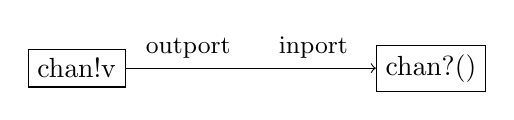
\begin{tikzpicture}
\draw (0,0) node[draw] (sender) {\scalashape chan!v};
\draw (4.5,0) node[draw] (receiver) {\scalashape chan?()};
\draw[->] (sender) -- 
  node[above,near start]{\small outport} 
  node[above,near end]{\small inport} (receiver);
\end{tikzpicture}
\end{center}

\item Values sent at the outport end (using |chan!v|) are received at the
  inport end (using |chan?()|), in the same order.

\item
Channels can be either synchronous or asynchronous; we will use a mix in this
course.
\end{itemize}
\end{slide}

%%%%%

\begin{slide}
\heading{Channels in SCL}

If |A| is a type, then \SCALA{Chan[A]} is the type of channels that pass data
of type~\SCALA{T}.  This has two subtypes:
%
\begin{itemize}
\item |SyncChan[A]|, of synchronous channels; 

\item |BuffChan[A]|, of buffered (or asynchronous) channels.
\end{itemize}

The command \SCALA{val chan = new SyncChan[A]} defines |chan| to be such a
synchronous channel.

The command \SCALA{chan!v} sends the value \SCALA{v} on \SCALA{chan}.

The expression \SCALA{chan?()} reads a value from~\SCALA{chan} and returns it.

The one that is executed first waits for the other; both then proceed.
\end{slide}

%%%%%

\begin{slide}
\heading{Channels in Scala}

The following two threads are equivalent (if \SCALA{x} and \SCALA{v} are
of type~\SCALA{A}): 
\begin{scala}
  { 
    val chan = new SyncChan[A]
    run(thread{ chan!v } || thread{ x = chan?() }) 
  }
\end{scala}
and
\begin{scala}
  x = v 
\end{scala}
\end{slide}

%%%%%


\begin{slide}
\heading{Example: copy}

Here's a thread that inputs values from the channel \SCALA{in}, and outputs
them on the channel~\SCALA{out}:
%
\begin{scala}
def copy[A](in: SyncChan[A], out: SyncChan[A]) = thread{
  while(true){ val x = in?(); out!x }
}
\end{scala}
%
(Note that the thread is parameterised by the channels, and by the type~|A|
of those channels.)

We could have written the body of \SCALA{copy} as simply:
\begin{scala}
  while(true) out!(in?()) 
\end{scala}
(Note that in both forms, the communication on |in| can proceed even if no
thread is ready to receive on |out|.)
\end{slide}

%%%%%

\begin{slide}
\heading{InPorts and OutPorts}

A channel is simply an \SCALA{InPort} (something from which threads can
receive) and an \SCALA{OutPort} (something on which threads can send):
%
\begin{scala}
  package ox.scl.channel

  trait InPort[A]  { def ?(): A; ... }
        
  trait OutPort[A] { def !(value: A): Unit; ... }
  
  trait Chan[A] extends InPort[A] with OutPort[A]{ ... }

  class SyncChan[A] extends Chan[A]{...} 
\end{scala}

The types \SCALA{InPort[A]} and \SCALA{OutPort[A]} can be abbreviated as
\SCALA{?[A]} and~\SCALA{![A]}.

Note that the terminology ``|InPort|'' and ``|OutPort|'' refer to the point of
view of \emph{threads}, not channels.
\end{slide}

%%%%%

\begin{slide}
\heading{InPorts and OutPorts}

\SCALA{copy} uses only the \SCALA{InPort} of \SCALA{in} and the
\SCALA{OutPort} of \SCALA{out}, so we could have written it as:
%
\begin{scala}
def copy[A] (in: ?[A], out: ![A]) = thread{ 
  while(true){ out!(in?()) } 
}
\end{scala}
%
Note how the signature makes it clear what the thread does with each
channel.  Also, this provides some type safety.
\end{slide}

%%%%%


\begin{slide}
\heading{More examples}

The following thread  repeatedly reads a
value from \SCALA{in} and writes it to standard output:
%
\begin{scala}
  def console[A](in: ?[A]) = thread{ while(true) println(in?()) }
\end{scala}

\SCALA{nats} sends the natural numbers to \SCALA{out}
%
\begin{scala}
  def nats(out: ![Int]) = thread{ 
    var n = 0; while(true){ out!n; n += 1 }
  }
\end{scala}

\SCALA{alts} copies alternate values read from \SCALA{in} to \SCALA{out}:
\begin{scala}
  def alts[A](in: ?[A], out: ![A]) = thread{ 
    while(true){ out!(in?()); in?() } 
  }
\end{scala}
\end{slide}

%%%%%

\begin{slide}
\heading{Example: printing multiples of four}

\begin{scala}
import ox.scl._

object Mults4{
  def console[A](in: ?[A]) = ...

  def nats(out: ![Int]) = ...

  def alts[A](in: ?[A], out: ![A]) = ...

  val x1, x2, x4 = new SyncChan[Int]

  def system = nats(x1) || alts(x1, x2) || alts(x2, x4) || console(x4)

  def main(args: Array[String]) = run(system)
}
\end{scala}
\end{slide}

%%%%%

\begin{slide}
\heading{Example: printing multiples of four}

\begin{center}
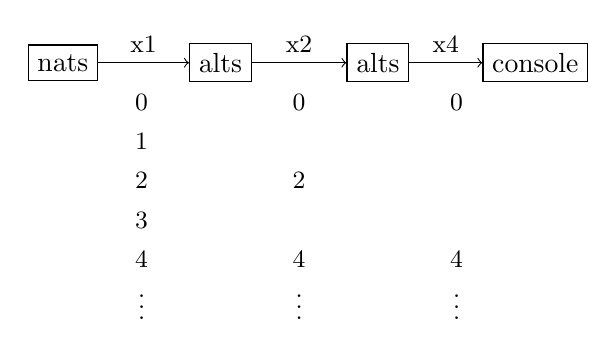
\begin{tikzpicture}
\draw (0,0) node[draw] (nats) {\scalashape nats};
\draw (nats)++(2,0) node[draw] (alts1) {\scalashape alts};
\draw[->] (nats) -- node[above]{\small\scalashape x1} (alts1);
\draw (alts1)++(2,0) node[draw] (alts2) {\scalashape alts};
\draw[->] (alts1) -- node[above]{\small\scalashape x2} (alts2);
\draw (alts2)++(2,0) node[draw] (console) {\scalashape console};
\draw[->] (alts2) -- node[above]{\small\scalashape x4} (console);
%
\draw (nats)++(1,-0.5) node {\small\scalashape 0};
\draw (nats)++(1,-1) node {\small\scalashape 1};
\draw (nats)++(1,-1.5) node {\small\scalashape 2};
\draw (nats)++(1,-2) node {\small\scalashape 3};
\draw (nats)++(1,-2.5) node {\small\scalashape 4};
\draw (nats)++(1,-3) node {\small\scalashape \vdots};
%
\draw (alts1)++(1,-0.5) node {\small\scalashape 0};
\draw (alts1)++(1,-1.5) node {\small\scalashape 2};
\draw (alts1)++(1,-2.5) node {\small\scalashape 4};
\draw (alts1)++(1,-3) node {\small\scalashape \vdots};
%
\draw (alts2)++(1,-0.5) node {\small\scalashape 0};
\draw (alts2)++(1,-2.5) node {\small\scalashape 4};
\draw (alts2)++(1,-3) node {\small\scalashape \vdots};
\end{tikzpicture}
\end{center}
\end{slide}

%%%%%

\begin{slide}
\heading{Buffered channels}

In the previous example, we used synchronous channels.  In effect, the send
and receive happen at the same time: the sender and receiver
\emph{synchronise} on the communication.

Using synchronous channels can make programs easier to understand: it helps us
to relate the states in different components.

By contrast, buffered channels allow a send to happen, even if there is no
thread ready to receive, up to some limit~|size| on the number of messages
that can be buffered.
\end{slide}

%%%%%

\begin{slide}
\heading{Buffered channels}

The class of buffered channels is defined as follows.\footnote{Internally, a
  {\scalashape BuffChan} stores the buffered messages in an array.  This means
  that the runtime implementation needs to construct an {\scalashape
    Array[A]}, so it needs to have a {\scalashape ClassTag} for~{\scalashape
    A}.  If {\scalashape A} is a concrete type, e.g.~{\scalashape Int}, then
  the runtime implementation can construct the {\scalashape ClassTag}.  But if
  {\scalashape A} is declared as a polymorphic type, it should be given the
  type bound {\scalashape A: scala.reflect.ClassTag}, and the compiler will
  ensure a {\scalashape ClassTag} is available.}
%
\begin{scala}
class BuffChan[A: scala.reflect.ClassTag](size: Int) extends Chan[A]
\end{scala}


\vfill
\end{slide}

%%%%%

\begin{slide}
\heading{Buffered channels}

In the multiples-of-four example, we could have defined the channels as 
%
\begin{scala}
  val x1, x2, x4 = new BuffChan[Int](10)
\end{scala}

Making the channels buffered might help to overcome inconsistencies in speed. 

Giving the channels some limit on buffering means that if the sender is faster
than the receiver, the buffer will not consume more and more memory.  
\end{slide}


% %%%%%

\begin{slide}
\heading{tee}

The following process inputs values on~\SCALA{in}, and outputs on
both~\SCALA{out1} and \SCALA{out2}.
%
\begin{scala}
def tee[A](in: ?[A], out1: ![A], out2: ![A]) = thread{
  while(true){ val v = in?(); out1!v; out2!v }
}
\end{scala}

The above version of \SCALA{tee} outputs on its \SCALA{out1} channel before
its \SCALA{out2} channel.  What happens if we use this in the context of some
larger system that inputs on \SCALA{out2} before \SCALA{out1}?  For example:
\begin{scala}
val in, out1, out2 = new SyncChan[Int]
run( tee(in, out1, out2) || thread{ println(out2?() + out1?()) } )
\end{scala}
\end{slide}

% %%%%%

\begin{slide}
\heading{tee}

Generic components should place as few assumptions as possible upon the
network in which they are placed.  The following version of |tee| performs the
outputs concurrently, i.e.~in either order.
%
\begin{scala}
def tee[A](in: ?[A], out1: ![A], out2: ![A]) = thread{
  while(true){ 
    val v = in?()
    run(thread{out1!v} || thread{out2!v}) 
  }
}
\end{scala}

However, creating and running two new threads is moderately expensive.  In
specific settings, it might be more efficient and easier to perform the
outputs in a fixed order.
\end{slide}

% %%%%%

\begin{slide}
\heading{Closing channels}

Often a component has to process a finite stream of data.  But how should the
end of the stream be signalled?
%
A way is for the sender to close the channel. 
%
It is also possible for a receiver to close a channel, to signal to the
sender that it is unable to accept more data. 

In SCL:
%
\begin{itemize}
\item If |in| is an |InPort| (e.g.~a channel), then |in.close| closes it.

\item If |out| is an |OutPort| (e.g.~a channel), then |out.endOfStream| closes
  it for sending. 
  \begin{itemize}
  \item For a synchronous channel, this also closes it for
  receiving.  
  \item For a buffered channel, other threads can continue to
  receive until the buffer becomes empty, at which point the channel becomes
  fully closed.
  \end{itemize}
\end{itemize}
\end{slide}

%%%%%

\begin{slide}
\heading{Dealing with closed channels}

If a thread tries to send or receive on a channel that has been closed, it
throws a |Closed| exception, a subclass of the |Stopped| exception class. 

Threads should normally catch such exceptions, and then do the right thing: in
many examples, it should close channels to other components, to signal to the
next component in line that the stream is closed.

%% If such closing is possible, the thread should handle it appropriately,
%% normally closing its channels to pass the message on. 
Here's a new version of
|alts| that does this.
%
\begin{scala}
def alts[A](in: ?[A], out: ![A]) = thread{ 
  try{ while (true) { out!(in?()); in?() } } 
  catch{ case _: Closed => in.close; out.endOfStream }
}
\end{scala}

Note: closing a channel that is already closed has no effect.

Note also that there's no need to close a channel that is about to go out of
scope and be garbage collected. 
\end{slide}

%%%%%
\begin{slide}
\heading{Closing channels}

The pattern on the previous slide is sufficiently common, that there's a
construct to capture it.  
%
\begin{scala}
  repeat{ <command> }
\end{scala}
%
behaves much like
\begin{scala}
  while(true){ <command> }
\end{scala}
but terminates (cleanly) if \SCALA{<command>} throws a \SCALA{Stopped}
exception.

For example:
%
\begin{scala}
def alts[A](in: ?[A], out: ![A]) = thread{ 
  repeat{ out!(in?()); in?() } 
  in.close; out.endOfStream
}
\end{scala}
\end{slide}

%%%%%

\begin{slide}
\heading{Closing channels}

The construct
%
\begin{scala}
  repeat(guard){ <command> }
\end{scala}
%
behaves much like
\begin{scala}
  while(guard){ <command> }
\end{scala}
but terminates (cleanly) if \SCALA{<command>} throws a \SCALA{Stopped}
exception.

A closed channel~|c| can be reopened using the construct
\begin{scala}
  c.reopen
\end{scala}
%
This has a precondition that the channel is indeed closed, and that no thread
is trying to send or receive on it.  This allows channels to be reused.

It is possible to test whether a channel is closed using
%
\begin{scala}
  c.isClosed
\end{scala}
\end{slide}


%%%%%

\begin{slide}
\heading{Summary}

\begin{itemize}
\item 
Message passing using channels;

\item
Synchronous channels, buffered channels, ports, sending and receiving;

\item
Closing channels; dealing with closed channels;

\item
Examples: components; pipelines; fine-grained concurrency.
\end{itemize}
\end{slide}


\end{document}
